
\chapter{对star\_tp和star-d的性能测试}
\label{chap:InSAR5}

\section{InSAR算法介绍}

InSAR\citep{wu2008insar}(Interferometric synthetic aperture radar, InSAR)即合成孔径雷达干涉技术最先在20世界60年代出现,在合成孔径雷达技术(SAR)的基础上,与射电天文学中的干涉测量技术相结合所形成的新技术。

InSAR 算法是合成孔径雷达技术(SAR)以及干涉测量技术的融合,利用传感器的数据参数以及成像几何关系等精确的测量地表上某个点的空间位置及其微小变化。InSAR算法是传统的SAR遥感技术与射电天文干涉技术相互结合而形成的新技术。InSAR算法利用雷达向目标区域发射微波,之后接收从目标反射回来的回波,从而得到对于同一区域的SAR复数图像对,同时,如果复图像之间存在相干条件,通过SAR复图像之间的共轭相乘,就可以得到干涉图,根据所得干涉图中的相位值,就可以得到两次成像中微波的路程差别,进而计算出目标地区的地形以及表面的微小变化,从而可以被用于数字高程模型的建立以及地壳形变的探测等。

InSAR算法在许多地学研究应用中都有很好的作用,利用InSAR进行全天候、高精度、高分辨率和数据处理高度自动化特征已经体现出来。InSAR算法在遥感制图、土地分类应用和大规模地形监测特别是细小地形监测方面具有广阔的前景。 

\section{InSAR算法基本原理}

InSAR测量模式主要分为两种:一种是双天线单轨(Single Pass)模式,该模式主要用于生成数字高程模型,一般被机载SAR所采用。另一种则是双轨(Two Pass) 模式,该模式主要用来获取地表的形变,一般被星载SAR所采用.我们用重复轨道干涉测量作为例子,简要介绍InSAR技术的基本原理,如图5.1所示。

\begin{figure}[!htbp]
    \centering
    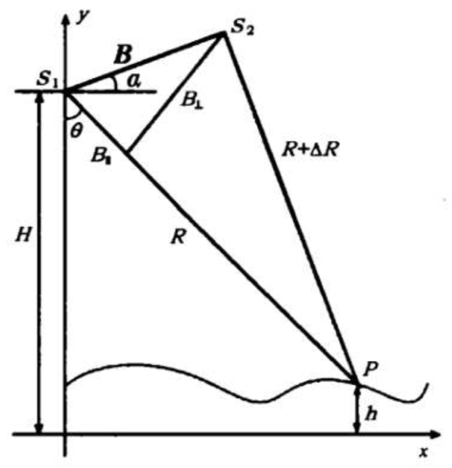
\includegraphics[width=0.40\textwidth]{5_insar_algo}
    \bicaption{InSAR基本原理。}{Fundamentals of InSAR.}
    \label{fig:5_insar_algo}
\end{figure}
 
在实际的测量过程中,卫星以不同的时间间隔以及不同程度的轨道偏离重复对某一区域成像,轨道偏离在几十米到一千米之间,假设在两次成像过程中,卫星处于不同的空间位置$S_1$和$S_2$,则空间干涉基线向量为$B$,其长度为$B$。基线向量$B$与水平方向的夹角为基线倾角$\alpha$。$S_1$和$S_2$到地面上点$P$的斜距分别是$R$和$R+\Delta R$,将基线沿视线方向分解,得到平行于和垂直于视线向的两个向量,$H$为到参考面的高度;从$S_1$发射波长为$\lambda$的信号经目标点$P$反射后被$S_1$接收,得到测量相位$\varphi_1$,

\begin{equation} \label{eq:eq1}
	\varphi_1=\frac{4\pi}{\lambda}R+arg\{u_1\}
\end{equation}

同样,另一个空间位置$S_2$上进行相同的测量会得到相位$\varphi_2$ ,

\begin{equation} \label{eq:eq2}
	\varphi_2=\frac{4\pi}{\lambda}(R+\Delta R)+arg\{u_2\}
\end{equation}

式中,$arg\{u1\}$和$arg\{u2\}$表示由于不同散射特性所造成的随机相位。如果假设两幅图像中随机相位的贡献值相同,则S1和S2关于目标P点的相位差则为公式5.3所示,

 \begin{equation} \label{eq:eq3}
	\varphi=\varphi_1-\varphi_2=-\frac{4\pi}{\lambda}\Delta R
\end{equation}

相位差也称为干涉相位,可由经过配准的两幅SAR SLC图共扼相乘得到。根据图5.1中的几何关系并利用余弦定理可得: 

\begin{equation} \label{eq:eq4}
	\sin(\theta-\alpha)=\frac{R^2+B^2-(R+\Delta R)^2}{2RB}
\end{equation}
\begin{equation} \label{eq:eq5}
	h=H-R\cos\theta
\end{equation}

5.4,5.5两式即为InSAR确定高程的原理性公式。

\section{InSAR数据处理的基本步骤}

InSAR算法数据处理的一般流程主要步骤包括西一下几个部分:影像配准、干涉图生成、噪声滤除、基线估算、平地效应去除、相位解缠、高程计算和纠正。如图5.2所示。InSAR算法属于遥感图像处理的系列算法,其典型应用就是遥感数据的处理以及地形变化的监测。 

\begin{figure}[!htbp]
    \centering
    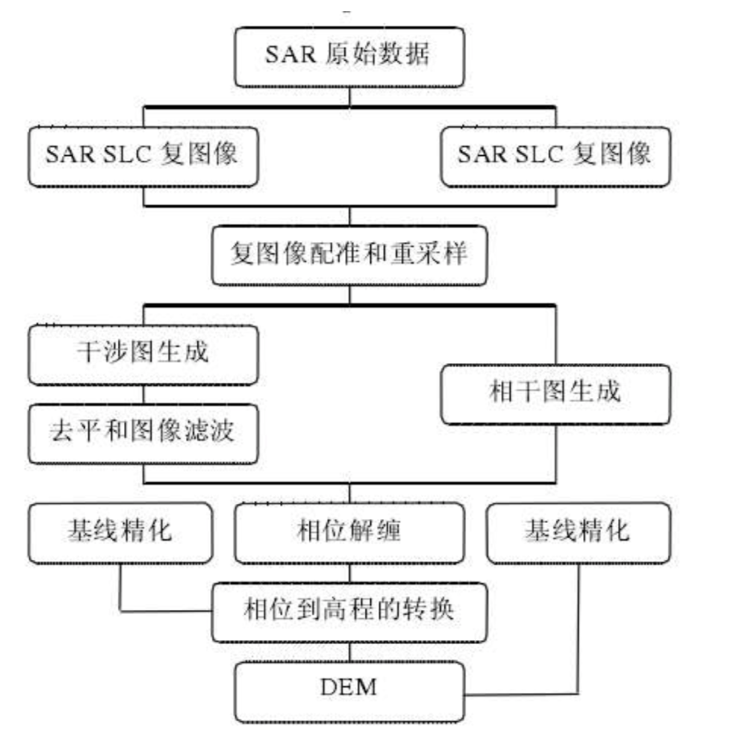
\includegraphics[width=0.40\textwidth]{5_insar_routine}
    \bicaption{InSAR数据处理的基本步骤。}{The basic data processing procedures in InSAR.}
    \label{fig:5_insar_routine}
\end{figure}

\section{InSAR算法分析和优化策略}

InSAR系列算法包括十几个图像处理算法以及若干数据辅助处理算法,算法的输入是多幅通过卫星遥感获得的TIF格式的图像数据,大小一般在3GB左右。整个算法的计算量较大,同时算法之间的依赖关系较为明显,并且在十几个算法的计算过程中,需要频繁的I/O操作,涉及到较多的大文件的读写,需要耗费大量的时间。一般InSAR算法的实现都是以满足功能和保证正确性以及精度为前提,在实际应用中计算效率较低,往往会成为科研过程的瓶颈,同时也给实时数据处理分析和决策带来了挑战,因此InSAR算法的优化工作是十分必要的。 

从高性能计算的角度分析,一般图像处理的算法具有较高的可并行性,并行化对于串行算法的性能升效果较好,特别是当前主流的服务器或者工作站都是基于多核架构,甚至是众核/加速器异构系统以及分布式系统,串行算法所能获得的性能较为有限,并行优化势在必行。 

通过对InSAR算法代码的分析以及对一般图像处理算法并行优化的调研,图像处理的并行化主要基于图像的分块处理,一般来说图像处理各图像块之间的依赖较为薄弱,可以通过优化手段达到较高的并行程度。例如共享内存环境下,通过将不同图像部分的计算映射到不同的处理器上,通过共享内存共享图像数据往往能获得较高的并行性能。对于算法内部的不同处理部分,分析其计算量,找到算法的计算瓶颈,进行重点优化。同时分析算法不同部分以及算法之间的依赖关系,对整个算法进行多层次的优化。同时对于I/O部分,要从两个方面进行优化,一方面将I/O操作并行化,解决串行I/O的瓶颈问题。另一方面,通过分析算法之间对于I/O操作的依赖,通过数据流的方式消除算法之间不必要的I/O操作,最大限度的提高程序性能。 

需要指出的是,对于算法的并行化并不是总是有效的,因为一般的图像处理算法虽然具有可并行性,但经常需要同步点或者需要通过加入互斥锁来保证并行的正确性,这样做会带来一定的性能损耗。有些算法例如精配准过程和干涉图像生成,其计算量相对较大,也既是有着较大的并行优化空间。有些程序如粗配准过程,其计算量相对较少,适合在单个处理器上串行处理。因此需要对整个算法流程进行计算量分析,优化性能瓶颈,同时需要感知计算环境,最优化分配计算资源,获得最高的加速比和程序性能。 

\section{InSAR并行优化实施方案}

\subsection{代码移植,找到计算热点}

将windows版本代码移植到linux平台上,使用gprof\citep{graham2004gprof}找到每个算法的计算核心。

一般来说,linux平台比windows平台更适合高性能程序的开发,在性能、稳定性、可编程性等方面都具有不小的优势,所以我们选择先将原始代码移植到linux平台,然后再进行并行优化。

并行优化的主要对象是算法的计算核心,即执行次数较多、耗时较长、占程序运行时间比例较大的代码段,通常表现为函数或代码段的循环调用。在使用并行优化工具和语言进行并行化之前,首先要找到计算核心,在本项目中,我们选择gprof工具来进行程序分析。gprof精确地给出函数被调用的时间和次数,给出函数调用关系。

\subsection{使用OpenMP对单个算法进行优化}

使用OpenMP对每个算法的计算核心(大部分是for循环)进行并行优化。

使用OpenMP时主要的困难在于要保证并行程序的线程安全,对临界区的访问要加锁保护。有时还要考虑将for循环之外的全局变量放到for循环之内,这样做的目的是减少线程同步的消耗,以空间换时间。

OpenMP的优势就是代码量比较小,只需要少量的制导语句就可以实现并行化。

\subsection{使用STAR系列工具对整个流程进行并行优化}

分析整个流程各个算法之间的依赖关系,使用自主研发的STAR系列并行优化工具(star\_tp和star-d)进行并行优化。InSAR算法的测试用例的任务拓扑图如图5.3所示。

\begin{figure}[!htbp]
    \centering
    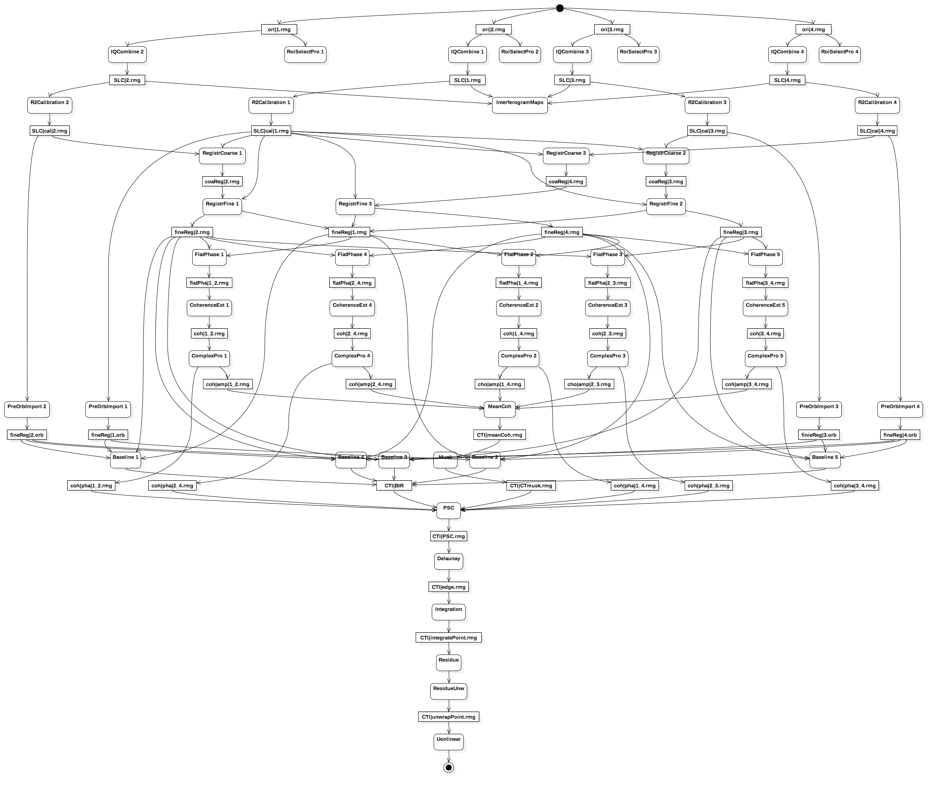
\includegraphics[width=1.0\textwidth]{5_insar_topo}
    \bicaption{InSAR测试用例的任务拓扑图。}{Topology of tasks in InSAR test case.}
    \label{fig:5_insar_topo}
\end{figure}

OpenMP的fork/join模式属于整体同步模型,存在大量的同步消耗,浪费CPU资源。STAR系列并行优化工具基于数据流模型,根据任务之间的依赖关系进行任务调度,实现了计算和通信的重叠,提高了CPU的利用效率,同时具有较好的可扩展性,从而实现更好的优化效果。

\section{优化结果}

\subsection{测试环境}

我们实验环境共有四台相同配置的服务器,每台服务器的测试环境如表5.1所示。除了star-d的测试需要同时用到四个节点以外,其他的测试都在一台服务器上完成。

\begin{table}[!htbp]
    \bicaption{InSAR测试环境。}{InSAR testing environment.}
    \label{tab:5_insar_test_env}
    \centering
    \footnotesize
    \setlength{\tabcolsep}{4pt}
    \renewcommand{\arraystretch}{1.2} 
    \begin{tabular}{|>{\bfseries}l|c|}
        \hline
        操作系统 & CentOS Linux release 7.3.1611 (Core) \\ \hline
        处理器 & Intel(R) Xeon(R) CPU E7- 8830  @ 2.13GHz \\ \hline
        核数 & 物理核数:8,逻辑核数:64 \\ \hline
        内存 & 1TB \\ \hline
        编译器 & gcc 4.8.5 \\ \hline
    \end{tabular}
\end{table}

测试用例的输入是四幅1.5GB的rmg格式的图像文件,输出是约60GB的图像文件和一些文本文件。

\subsection{linux版本基准测试结果}

表5.2的“串行”一列是windows版本移植到Linux平台后的串行程序测试结果。其中部分算法的计算量特别小,没有优化的必要,后续的优化重点关注加粗部分的算法的优化效果,包括一下算法:R2Calibration、RegistrFine、FlatPhase、CoherenceEst、ComplexPro、Baseline和Delaunay。

\subsection{寻找计算核心}

\begin{figure}[!htbp]
    \centering
    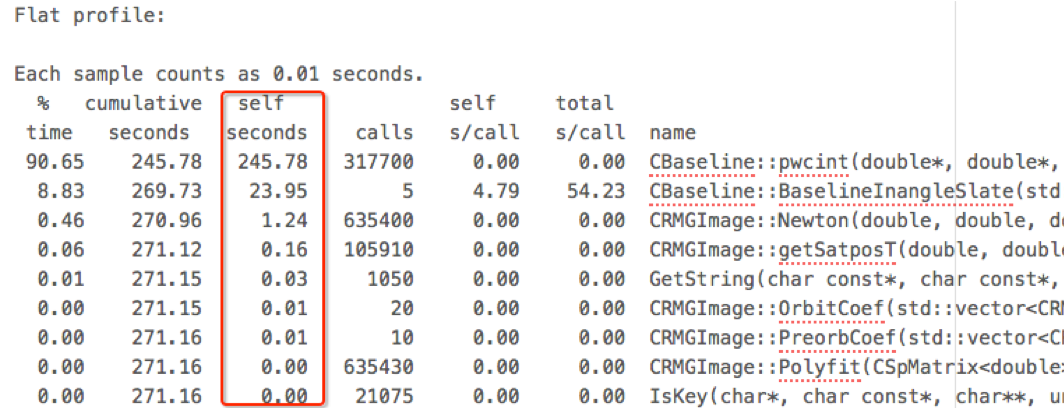
\includegraphics[width=0.60\textwidth]{5_insar_linux_gprof}
    \bicaption{Baseline算法的gprof日志。}{Gprof log of Baseline algorithm.}
    \label{fig:5_insar_linux_gprof}
\end{figure}

得到稳定的linux版本后,要寻找各个算法的计算热点。我们采用的工具是gprof,在程序编译的时候加入gprof选项,程序运行结束后会产生gprof的日志文件。

以Baseline算法为例,图5.4是使用gprof得到的日志,可以看出,pwcint()函数和BaselineInageleSlate()函数占了99%以上的运行时间,应该重点优化这两个函数。

其他的算法以通样的方式找到计算核心,然后重点针对计算核心进行优化。

\subsection{OpenMP版本优化结果}

表5.2是OpenMP版本的单元测试结果和整个流程运行时间结果。

\begin{table}[!htbp]
    \bicaption{OpenMP版本的InSAR算法测试结果。}{Result of OpenMP version InSAR.}
    \label{tab:5_insar_openmp_result}
    \centering
    \footnotesize
    \setlength{\tabcolsep}{4pt}
    \renewcommand{\arraystretch}{1.2} 
    \begin{tabular}{|l|c|c|c|c|c|c|c|c|c|c|}
        \hline
	\diagbox{算法}{线程数}  &   \texttt{串行}	&   1	    &   2	    &   4	    &   8	    &   10	    &   12	    &   16	    &   32	    &   64      \\ \hline
		IQCombine	        &   8.74	&   10.85	&   5.90	&   5.01	&   5.24	&   5.03	&   5.48	&   5.14	&   5.56	&   7.68      \\ \hline
		R2Calibration	    &   32.97	&   33.84	&   19.01	&   9.86	&   8.65	&   8.68	&   8.75	&   8.79	&   9.11	&   10.33      \\ \hline
		InterferogramMaps	&   0.01	&   0.01	&   0.01	&   0.01	&   0.01	&   0.01	&   0.01	&   0.01	&   0.01	&   0.01      \\ \hline
		RegistrCoarse	    &   14.66	&   20.74	&   10.72	&   6.44	&   6.57	&   6.60	&   6.62	&   6.71	&   6.85	&   7.96      \\ \hline
		RegistrFine	        &   246.68	&   278.36	&   149.55	&   81.89	&   50.73	&   47.46	&   39.20	&   39.59	&   34.99	&   34.39      \\ \hline
		PreOrbImport	    &   0.46	&   0.46	&   0.45	&   0.46	&   0.45	&   0.45	&   0.46	&   0.46	&   0.46	&   0.47      \\ \hline
		RoiSelectPro	    &   0.13	&   0.12	&   0.13	&   0.14	&   0.13	&   0.14	&   0.13	&   0.13	&   0.13	&   0.12      \\ \hline
		FlatPhase	        &   114.35	&   126.31	&   67.34	&   36.38	&   20.27	&   17.44	&   15.63	&   14.74	&   16.11	&   23.96      \\ \hline
		CoherenceEst	    &   296.59	&   313.01	&   159.11	&   80.00	&   40.38	&   34.03	&   27.33	&   22.73	&   24.64	&   27.85      \\ \hline
		ComplexPro	        &   26.60	&   27.10	&   13.72	&   6.92	&   3.52	&   2.84	&   2.49	&   2.39	&   2.61	&   3.39      \\ \hline
		MeanCoh	            &   0.23	&   0.23	&   0.18	&   0.16	&   0.15	&   0.14	&   0.14	&   0.14	&   0.15	&   0.15      \\ \hline
		Musk	            &   0.35	&   0.36	&   0.33	&   0.29	&   0.28	&   0.28	&   0.28	&   0.28	&   0.28	&   0.21      \\ \hline
		Baseline	        &   272.60	&   273.81	&   140.07	&   71.74	&   37.29	&   30.43	&   25.87	&   20.07	&   11.95	&   8.60      \\ \hline
		PSC	                &   15.54	&   15.73	&   15.67	&   15.72	&   15.46	&   15.56	&   16.95	&   15.60	&   15.68	&   18.22      \\ \hline
		Delaunay	        &   52.70	&   52.90	&   41.76	&   36.52	&   33.31	&   33.24	&   32.34	&   32.28	&   35.71	&   40.76      \\ \hline
		Integration	        &   3.55	&   3.62	&   3.58	&   3.60	&   3.63	&   3.67	&   3.61	&   3.59	&   3.59	&   3.58      \\ \hline
		Residue	            &   1.13	&   1.21	&   1.40	&   1.54	&   1.90	&   1.88	&   2.31	&   2.20	&   3.20	&   3.50      \\ \hline
		ResidueUnw	        &   0.26	&   0.28	&   0.27	&   0.26	&   0.27	&   0.27	&   0.26	&   0.27	&   0.27	&   0.27      \\ \hline
		Uonlinear	        &   11.22	&   10.28	&   6.81	&   4.50	&   4.02	&   3.50	&   3.79	&   3.76	&   3.76	&   4.58      \\ \hline
        总运行时间(秒) 	&   1098.77	&   1169.22	&   636.01	&   361.44	&   232.26	&   211.65	&   191.65	&   178.88	&   175.06	&   196.03      \\ \hline
    \end{tabular}
\end{table}

单个算法的加速比由2倍到20多倍不等,这种差异是由算法本身的特点决定的,计算密集型的算法(如Baseline)的加速比可以达到20多倍,I/O密集型的算法(如IQCombine)的加速比只有不到2倍。

\begin{figure}[!htbp]
    \centering
    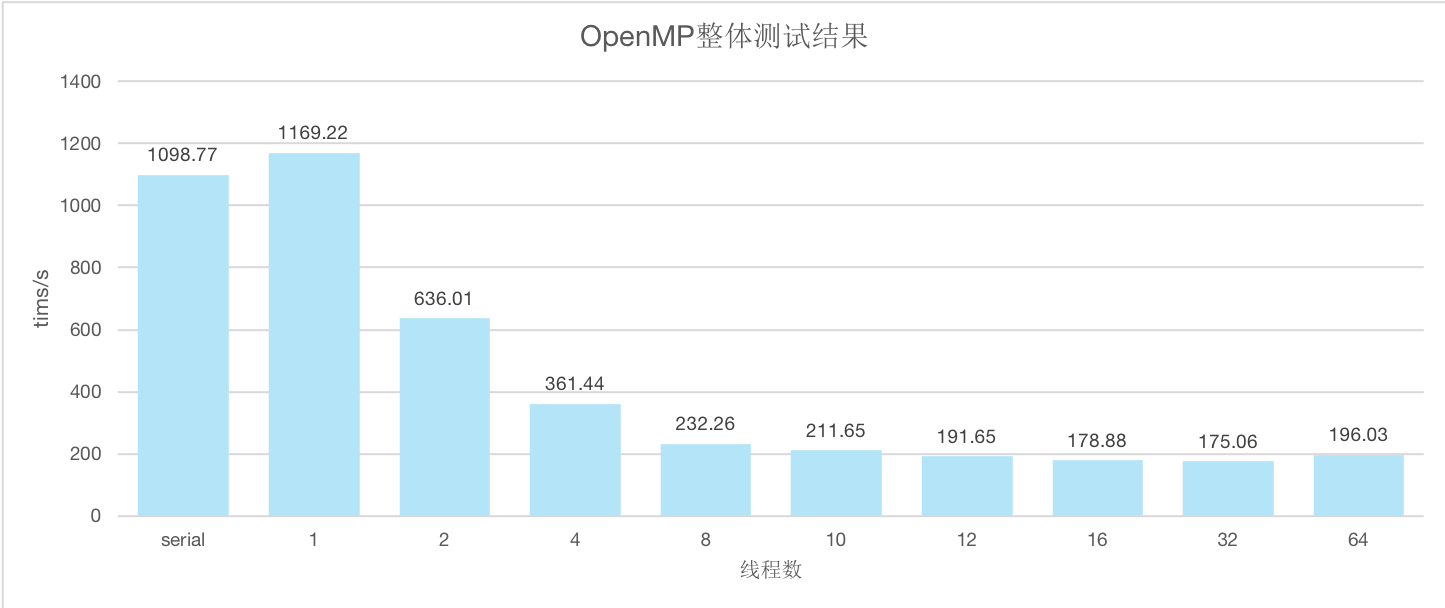
\includegraphics[width=0.80\textwidth]{5_insar_openmp_result}
    \bicaption{OpenMP版本InSAR整个流程性能优化结果。}{Performance of InSAR overall routines on OpenMP version.}
    \label{fig:5_insar_openmp_result}
\end{figure}

图5.5是OpenMP版本整个流程的加速比,在开启32线程时达到6倍左右,之后随着线程数增加,操作系统管理线程的开销过大,导致性能开始下降。

\subsection{star\_tp优化结果}

将OpenMP版本的函数进一步封装成star\_tp中的task,进行整体流程的进一步优化,图5.6是star\_tp版本与OpenMP版本的整体流程优化效果的对比。

\begin{figure}[!htbp]
    \centering
    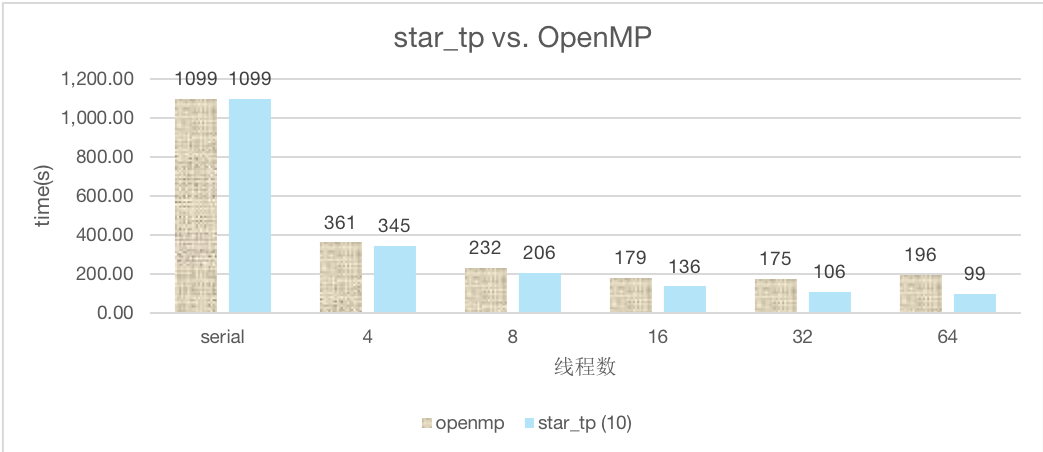
\includegraphics[width=1.0\textwidth]{5_insar_star_tp_openmp}
    \bicaption{star\_tp与OpenMP的对比。}{star\_tp vs. OpenMP.}
    \label{fig:5_insar_star_tp_openmp}
\end{figure}

测试中star\_tp的线程池的容量设置为10(根据最大并行度来设置,从图5.3可以粗略估计出最大并行度)。通过图5.6可以看出,线程数相同时,star\_tp的优化效果要优于OpenMP,而且当线程数由32增加为64时,OpenMP版本的性能开始下降,而star\_tp的性能还在提升,这体现出了star\_tp更高的CPU利用率;从最好的优化效果看,star\_tp对InSAR的加速比最高达到将近11倍,超过了OpenMP版本的6倍。

\subsection{star-d优化结果}

star-d的开发和测试依赖nfs,使用nfs作为分布式文件系统会导致算法中I/O时间与计算时间的比例发生很大变化。所以首先在nfs上运行了InSAR算法的linux版本和OpenMP版本,得到在本地环境下和nfs下I/O时间与计算时间的比例的对比(如表5.3),还有OpenMP版本和star-d版本在nfs下的测试结果(如表5.4)。

\begin{table}[!htbp]
    \bicaption{linux版本的InSAR算法在本地I/O和nfs下计算时间与I/O时间的比例。}{Comparison of computing time and I/O time of linux version InSAR with local I/O and nfs.}
    \label{tab:5_insar_openmp_result}
    \centering
    \footnotesize
    \setlength{\tabcolsep}{4pt}
    \renewcommand{\arraystretch}{1.2} 
    \begin{tabular}{|l|c|c|}
        \hline
        			&   I/O		& 	compute	\\ \hline
		local I/O	&   87		&   989		\\ \hline
		nfs			&	1002	&   989		\\ \hline
    \end{tabular}
\end{table}

\begin{table}[!htbp]
    \bicaption{OpenMP版本和star-d版本的InSAR算法在nfs上的测试结果。}{Result of OpenMP version and star-d version of InSAR on nfs.}
    \label{tab:5_insar_openmp_result}
    \centering
    \footnotesize
    \setlength{\tabcolsep}{4pt}
    \renewcommand{\arraystretch}{1.2} 
    \begin{tabular}{|l|c|c|c|c|c|}
        \hline
 \diagbox{版本}{线程数} &   1       &   4       &   8       &   16      \\ \hline
    OpenMP	            & 	1954.03	& 	1228.37	& 	1128.04	&	1078.40 \\ \hline
    star-d	            & 	1265.09	& 	1140.34	& 	1057.34	&	1027.32 \\ \hline
    \end{tabular}
\end{table}

为了得到更加真实的优化效果,我们去掉nfs下1002s的I/O时间,得到OpenMP版本和star-d版本的InSAR算法的计算时间的对比,如表5.5。

\begin{table}[!htbp]
    \bicaption{OpenMP版本和star-d版本的InSAR算法在nfs上的计算时间对比。}{Computing time of OpenMP version and star-d version of InSAR on nfs.}
    \label{tab:5_insar_openmp_result}
    \centering
    \footnotesize
    \setlength{\tabcolsep}{4pt}
    \renewcommand{\arraystretch}{1.2} 
    \begin{tabular}{|l|c|c|c|c|c|}
        \hline
 \diagbox{版本}{线程数} &   1       &   4       &   8       &   16      \\ \hline
    OpenMP	            & 	952.03	& 	226.37	& 	126.04	&	76.40	\\ \hline
    star-d	            & 	263.09	& 	138.34	& 	55.34	&	25.32 \\ \hline
    \end{tabular}
\end{table}

star-d和OpenMP的优化效果的对比如图5.7所示。

\begin{figure}[!htbp]
    \centering
    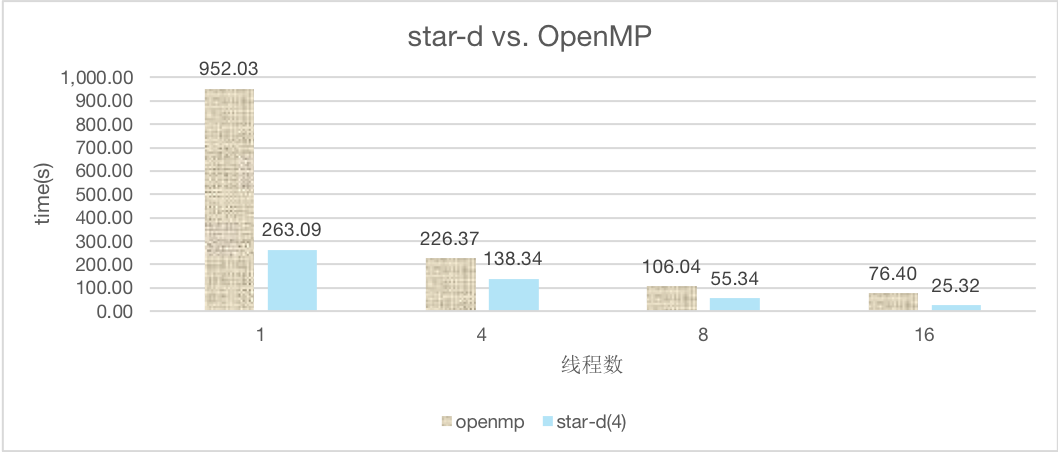
\includegraphics[width=1.0\textwidth]{5_insar_star-d_openmp}
    \bicaption{star-d与OpenMP的对比。}{star-d vs. OpenMP.}
    \label{fig:5_insar_star-d_openmp}
\end{figure}

测试中,star-d的worker个数设置为4,每个worker执行任务时开启与OpenMP版本相同的线程数。从计算时间上看,与OpenMP单线程测试结果相比,开启16个线程时,OpenMP达到12倍的加速比,star-d达到38倍的加速比。即使用4个worker的时候,star-d达到了OpenMP版本的3倍以上的性能,这是star-d的可扩展性的表现。
